\documentclass[sigconf,screen,9pt]{acmart}

% Flag to disable all editing macros and make the document ready for
%  submission.
\newif\ifEditMode

% Editing mode.
\EditModetrue
% % Submission mode.
% % The `submission' mode merges certain comments and edits, and removes some
% % other notes, TODOs and remarks. For more details, refer to the `reviewing
% % macros' in the `vusec.sty' file.
% \EditModefalse


\usepackage{vusec}
\usepackage{frontmatter}
\usepackage{aliases}


\begin{document}


%% Thesis title.
\newcommand{\thesistitle}{My Thesis: what, why, and how?}


%% Author information.
%% (Used in a couple of places, so it's better to define them in one place.)
\newcommand{\thauthor}{Anonymous Penguin}
%%  Student number.
\newcommand{\thauthorid}{007}
\newcommand{\thauthoremail}{anonpenguin@student.vu.nl}
\newcommand{\thauthoraff}{Vrije Universiteit Amsterdam}


%% Thesis type.
%% Valid values are `vubachelor', `csmaster', `pdcsmaster', `csecmaster', and `litstudy'.
%%
\thtype{csecmaster}

%% Course code.
% \thcc{0123}

%% Thesis title.
\thtitle{\thesistitle}

%% Paper/thesis author.
\thauthname{\thauthor}
\thauthid{\thauthorid}

%% First supervisor.
% \thsvfirst{First supervisor's name}{First supervisor's title}

%% Daily supervisor.
% \thsvdaily{Daily supervisor's name}{Daily supervisor's title}

%% Second reader.
% \thrdrsecond{Second reader's name}{Second reader's title}

\pagenumbering{gobble}
%% Attach customize front matter.
\addfrontmatter{}


\title{\thesistitle}

\author{\thauthor}
\affiliation{
  \institution{\thauthoraff}
  \city{Amsterdam}
  \country{NL}
}
\email{\thauthoremail}


\begin{abstract}
This paper describes a project that aims to create a low-noise kernel in order to demonstrate cpu attacks that make use of a side channel. Attacks which make use of a side channel can be complicated by channel interference and so this project aims to minimise those complications.
We will first give a high level overview of the system followed by a more detailed look at the design of the kernel and discuss various advantages and disadvantages each design decision entails afterwhich we will briefly go over the implementation of the kernel. From there we will move on to two example attacks that can be performed, flush + reload and spectre. Finally we will evaluate the kernel, discuss related.... THIS SHOULD BE WRITTEN LAST 

%%% Local Variables:
%%% mode: latex
%%% TeX-master: "../thesis"
%%% End:

\end{abstract}

\maketitle

\pagenumbering{arabic}

\section{Introduction}\label{s:intro}

\TODO{
This section includes some motivations behind the work, explicitly or implicitly
highlights the research question, provides a high-level explanation of the
solution, and describes the contributions.
}


\lipsum[1-2]

\begin{figure}[bh]
    %% The macro `\onecolgrid' is defined in `vusec.sty'
    %% NOTE: The suffix "./figs/" is implicitly included for this relative path.
    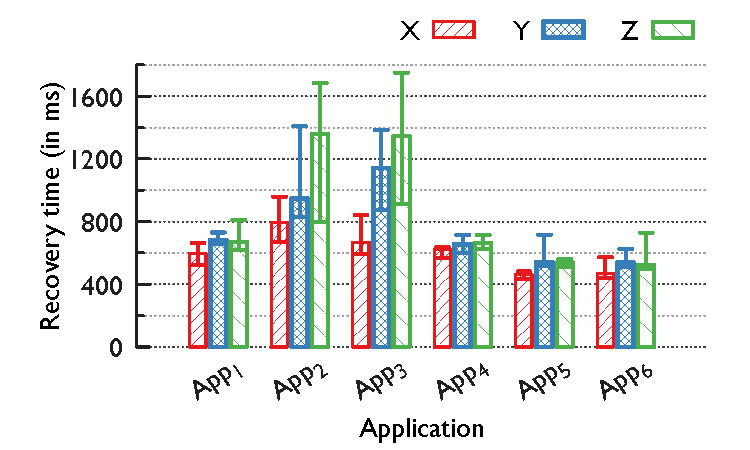
\includegraphics[width=\onecolgrid]{cache-by-app}
    %% Labels should immediately follow caption, to keep latex quiet.
    \figcap{Simple one-column figure. Please include a brief explanation or
    takeaway.}\label{fig:1col}
\end{figure}

\lipsum[3-4]

\begin{figure*}[th]
    %% The macro `\threecolgrid' is defined in `vusec.sty'
    \begin{subfigure}[t]{\threecolgrid}
        %% NOTE: The suffix "./figs/" is implicitly included for these relative paths.
        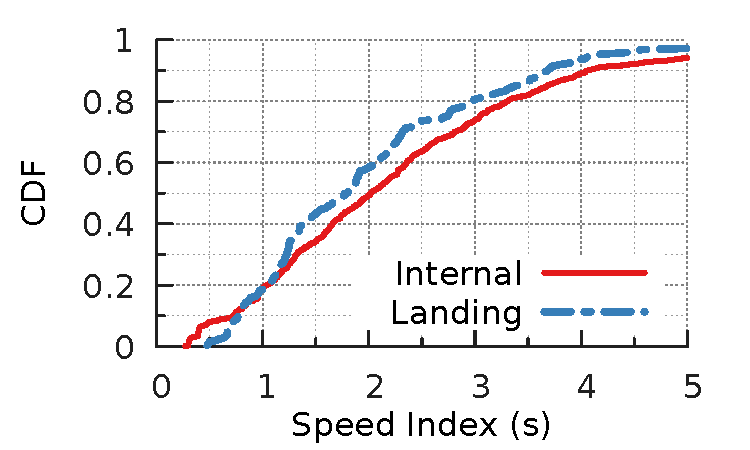
\includegraphics[width=\linewidth]{three-col/speed_index}
        \sfigcap{}\label{fig:3col-a}
    \end{subfigure}
    \begin{subfigure}[t]{\threecolgrid}
        %% NOTE: You do not have to mention the extension.
        %% (The example figures are in PDF format.)
        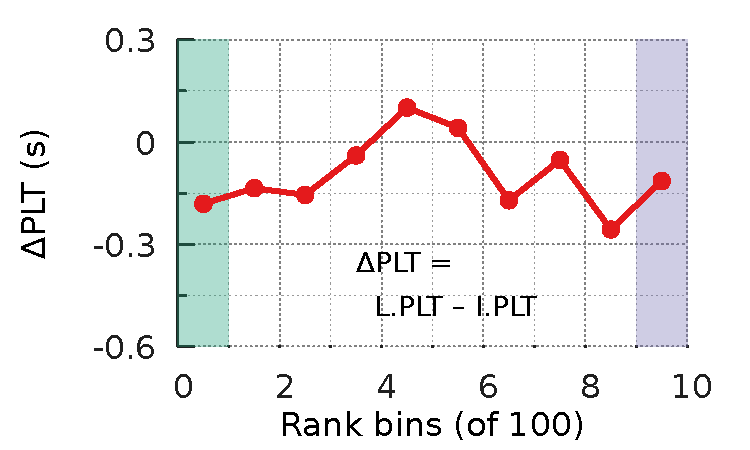
\includegraphics[width=\linewidth]{three-col/plt_ranks_diff}
        \sfigcap{}\label{fig:3col-b}
    \end{subfigure}
    \begin{subfigure}[t]{\threecolgrid}
        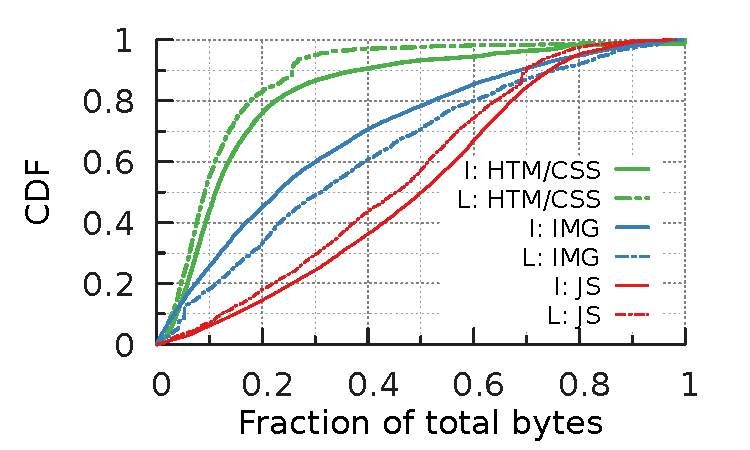
\includegraphics[width=\linewidth]{three-col/mimes}
        \sfigcap{}\label{fig:3col-c}
    \end{subfigure}
    %% Labels should immediately follow caption, to keep latex quiet.
    \figcap{Generate clear and beautiful figures (in PDF) that can be rendered side by side while still being easy to read and interpret. Choose colors wisely from the colorbrewer2.org website.}\label{fig:3col}
\end{figure*}

\lipsum[6-8]

\begin{table}[hb]
    \centering
    \tabcap{A simple table describing the characteristics of a data set or the
    results of an experiment.}\label{tab:sample}
    \taburulecolor{black!45}
    \begin{tabu}{c|c|r|r|r|r}
        \toprule
        \multirow{2}{*}{\thead{Char.}} &
            \multirow{2}{*}{\thead{\#samples}} &
            \thead{Count} &
            \multicolumn{3}{c}{\thead{Perf. Score}}\\
        &
            &
            \thead{of items} &
            \thead{X} & \thead{Y} & \thead{Z} \\
        \midrule
        \stress{P}
            & 214 & 56 & 9 & 23 & 24 \\
        \stress{Q}
            & 117 & 27 & 7 & 10 & 10 \\
        \stress{R}
            & 222 & 11 & 6 & 4 & 1 \\
        \stress{S}
            & 187 &  9 & 1 & 6 & 2 \\
        \stress{T}
            & 180 & 16 & 7 & 5 & 4 \\
        \bottomrule
    \end{tabu}

\end{table}

\lipsum[12-18]

\TODO{
We summarize our contributions as follows.
}

\case{}
%
\lipsum[10][1-2]

\case{}
% 
\lipsum[11][3-4]

\case{}
% 
\lipsum[12][5-6]


%%% Local Variables:
%%% mode: latex
%%% TeX-master: "../thesis"
%%% End:

\section{Background}\label{s:background}


\TODO{
This section provides the necessary context to help the reader understand the
remainder of the thesis.
}

\lipsum[1-8]


%%% Local Variables:
%%% mode: latex
%%% TeX-master: "../thesis"
%%% End:

\section{Threat Model}\label{s:threat-model}


\TODO{
Use this section to address key questions: (a) What does this thesis or paper
assume about the attackers’ goals and objectives? (b) What do you assume about
the systems and their environment, etc.
}

\lipsum[1-6]


%%% Local Variables:
%%% mode: latex
%%% TeX-master: "../thesis"
%%% End:

\section{Overview}\label{s:overview}


\TODO{
This section provides a high-level outline of the proposed system or solution.
It typically illustrates the system architecture or the interactions between the
different solution components (via a “boxes-and-arrows” diagram) from a user’s
perspective.
}


\lipsum[1-6]


%%% Local Variables:
%%% mode: latex
%%% TeX-master: "../thesis"
%%% End:

\section{Design}\label{s:design}


\TODO{
In this section, you would provide a high-level description of the system or
solution and explain your design choices.
}


\lipsum[1-10]


%%% Local Variables:
%%% mode: latex
%%% TeX-master: "../thesis"
%%% End:

\section{Evaluation}\label{s:evaluation}


\TODO{
Discuss the design of your experiments, the results you obtained, and how they
help in evaluating the claims you made in the introduction. You may also use the
evaluation results in this section to justify your design choices or assess the
contributions of different aspects  of your design towards the overall goals.
}


\lipsum[1-16]


%%% Local Variables:
%%% mode: latex
%%% TeX-master: "../thesis"
%%% End:

\section{Discussion}\label{s:discussion}


\TODO{
A “limitations” section, as the name implies, describes scenarios where the
proposed solution may not work well. Although a “discussion” section could also
highlight limitations of the proposed work, it focuses on analyzing the
implications of the proposed work for current and future research.
}


\lipsum[1-8]


%%% Local Variables:
%%% mode: latex
%%% TeX-master: "../thesis"
%%% End:

\section{Related Work}\label{s:related}


\TODO{
It is quite unlikely that you were the first to address this problem. Please use
this section, hence, to discuss what prior work had done and how your solution
is different from or better than prior work. You may place this section
immediately after the “Background” section, if necessary.
}


\lipsum[14-17][4-8]


\TODO{
Srinivasan Keshav's old---but still relevant---article on how to read a paper is an
excellent read in general for performing literature
surveys~\cite{Keshav-SIGCOMMCCR2007}.
}


%%% Local Variables:
%%% mode: latex
%%% TeX-master: "../thesis"
%%% End:

\section{Conclusion}\label{s:conclusion}


\TODO{
Briefly summarize your contributions, and share a glimpse of the implications of
this work for future research.
}


\lipsum[1-2]


%%% Local Variables:
%%% mode: latex
%%% TeX-master: "../thesis"
%%% End:


\bibliographystyle{ACM-Reference-Format}
\bibliography{references}

\end{document}


%%% Local Variables:
%%% mode: latex
%%% TeX-master: t
%%% End:
